% Part 2: Mixture of Experts, the BERT backbone, WEMoE and the FSFT objective.
\section{Method}

\begin{frame}{Idea: Mixture of Experts}
  \begin{columns}[c]
    \begin{column}{.36\linewidth}
      \centering
      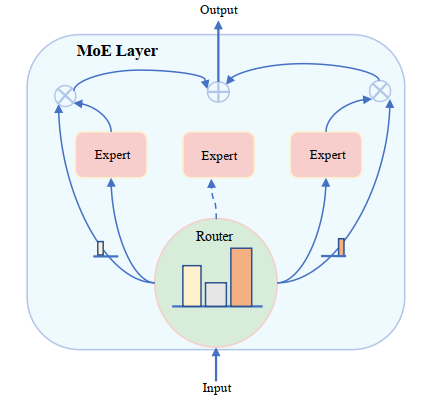
\includegraphics[height=3.3cm]{arch_moe}\\[-1mm]
      {\tiny Mixture of Experts layer\refm{6}}
    \end{column}
    \begin{column}{.62\linewidth}
      \[\mathrm{MoE}(x)=C\big(\{G_i(x)\cdot E_i(x)\}_{i=1}^{n}\big)\]
      \begin{itemize}
        \item Router $G$ decides how much each expert counts for \textbf{this input}.\refm{1}
        \item That is exactly the dynamic behaviour the problem asks for.
      \end{itemize}
    \end{column}
  \end{columns}
  \vfill
  \begin{block}{From outputs to weights}
    Running every expert is what we want to avoid. \textbf{WEMoE} mixes experts in \textbf{weight space}: the expert is a task vector, and one forward pass is enough.\refm{2}
  \end{block}
  \nextq{which backbone do we merge?}
\end{frame}

%% ---------- PART 3: THEORY ----------
\begin{frame}{BERT encoder: the shared backbone}
  \centering
  \begin{tikzpicture}[x=1cm,y=1cm]
    % full model
    \node[plain] (x) at (.75,0) {Tokens $x$: \texttt{[CLS]} $A$ \texttt{[SEP]}\\ (+ $B$ \texttt{[SEP]} for pairs)};
    \node[frz,minimum width=2.35cm] (emb) at (3.75,0) {Embeddings\\ token + segment + position\\ then LayerNorm};
    \node[frz,minimum width=2.3cm,very thick] (enc) at (6.75,0) {\textbf{Encoder layer} $\ell$\\ repeated $\times 12$};
    \node[frz,minimum width=1.75cm] (pool) at (9.2,0) {Pooler\\ {[CLS]}: dense, tanh};
    \node[frz,minimum width=1.6cm] (head) at (11.35,0) {Head $g_t$\\ dropout, linear};
    \node[plain] (out) at (13.1,0) {Logits\\ $\to\hat y$};
    \foreach \a/\b in {x/emb,emb/enc,enc/pool,pool/head,head/out} \draw[flow] (\a) -- (\b);
    % one encoder layer
    \node[plain] (in) at (.55,-1.75) {$h$};
    \node[frz,minimum width=1.9cm] (att) at (2.25,-1.75) {Multi-head\\ self-attention};
    \node[frz,minimum width=.95cm] (an1) at (4.2,-1.75) {Add\\ \&Norm};
    \node[mix,minimum width=1.2cm] (fc1) at (6.05,-1.75) {Linear\\ $W_1,b_1$};
    \node[frz,minimum width=.85cm] (act) at (7.5,-1.75) {GELU};
    \node[mix,minimum width=1.2cm] (fc2) at (8.95,-1.75) {Linear\\ $W_2,b_2$};
    \node[frz,minimum width=.95cm] (an2) at (10.85,-1.75) {Add\\ \&Norm};
    \node[plain] (outh) at (12.4,-1.75) {$h'$};
    \foreach \a/\b in {in/att,att/an1,an1/fc1,fc1/act,act/fc2,fc2/an2,an2/outh} \draw[flow] (\a) -- (\b);
    % residual connections
    \coordinate (r1) at ($(in.east)!.45!(att.west)$);
    \coordinate (r2) at ($(an1.east)!.45!(fc1.west)$);
    \draw[flow] (r1) -- ++(0,.62) -| (an1.north);
    \draw[flow] (r2) -- ++(0,.62) -| (an2.north);
    % groups
    \begin{scope}[on background layer]
      \node[group,draw=hustamber,thick,fit=(fc1)(act)(fc2)] (mlp) {};
      \coordinate (ltop) at ($(r1)+(0,.62)$);
      \coordinate (lbot) at ($(mlp.south)+(0,-.3)$);
      \node[group,inner sep=5pt,fit=(in)(outh)(att)(an2)(ltop)(lbot)] (lay) {};
    \end{scope}
    \draw[hustgray,dotted,thick] (enc.south west) -- (lay.north west);
    \draw[hustgray,dotted,thick] (enc.south east) -- (lay.north east);
    % labels
    \node[font=\scriptsize\bfseries,text=hustamber!85!black,anchor=north] at (mlp.south) {MLP block: its linear layers are upscaled later by WEMoE};
    \node[note,anchor=north west] at ([yshift=-1pt]lay.south west) {\scriptsize $h'=\mathrm{LayerNorm}\big(h+\mathrm{Sublayer}(h)\big)$};
    \node[note,anchor=north east] at ([yshift=-1pt]lay.south east) {\scriptsize $\mathrm{MLP}(h)=W_2\,\mathrm{GELU}(W_1h+b_1)+b_2$};
  \end{tikzpicture}
  \vfill
  \raggedright
  \begin{itemize}\footnotesize
    \item \texttt{bert-base-uncased}: 12 encoder layers, 109.5M parameters.\refm{3} All experts share this structure, so weights can be subtracted and added position by position.
    \item Self-attention gives each token a state that reflects its whole context. The {[CLS]} state passes through the pooler to the head of task $t$.
    \item CoLA and SST-2 use a single sentence; MRPC, RTE and QNLI use a sentence pair.
  \end{itemize}
  \nextq{how is this structure merged?}
\end{frame}

\begin{frame}{WEMoE architecture: two kinds of merging}
  \centering
  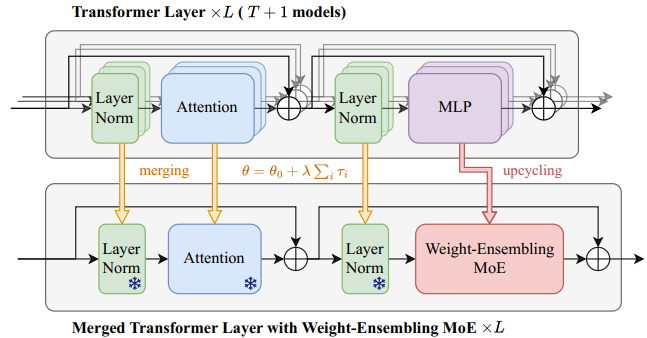
\includegraphics[height=3.35cm]{arch_wemoe_overview}\\[-.5mm]
  {\tiny Top: the fine-tuned and pretrained models. Bottom: the merged layer.\refm{2}}
  \vfill
  \raggedright
  \begin{itemize}\footnotesize
    \item \textbf{Static:} weights outside the MLP are merged once with Task Arithmetic. In this project that also covers embeddings and pooler.
    \item \textbf{Dynamic:} each MLP is upscaled to a Weight-Ensembling MoE module, so its weights depend on the input.
    \item Frozen parts carry the snowflake mark; only the router will be trained.
  \end{itemize}
  \nextq{first the static part, then the module.}
\end{frame}

\begin{frame}{Task Arithmetic: static merge with task vectors}
  \begin{columns}[c]
    \begin{column}{.3\linewidth}
      \centering
      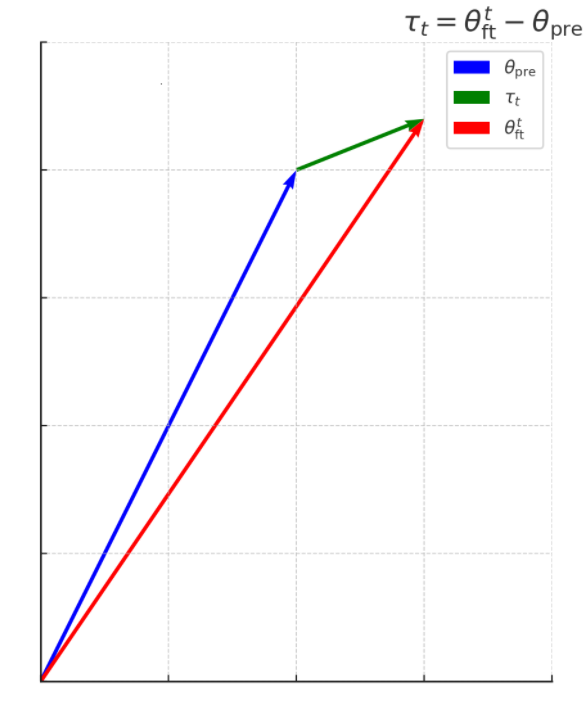
\includegraphics[height=3.6cm]{arch_task_vector}
    \end{column}
    \begin{column}{.68\linewidth}
      \textbf{Task vector:} what fine-tuning changed for task $i$\refm{4}
      \[\tau_i=\theta_i-\theta_0\qquad(\theta_{\mathrm{pre}}=\theta_0,\ \ \theta_{\mathrm{ft}}^{\,i}=\theta_i)\]
      \textbf{Task Arithmetic:} add the vectors back to the base
      \[\theta=\theta_0+\lambda\sum_{i=1}^{n}\tau_i\]
    \end{column}
  \end{columns}
  \vfill
  \begin{itemize}\footnotesize
    \item $\lambda$ controls how strongly the task vectors contribute; it is chosen on dev.
    \item Simple and compact, but the result is the same for every input.
  \end{itemize}
  \nextq{make the coefficients depend on the input, in the MLPs.}
\end{frame}

\begin{frame}{Router and WEMoE module: input-conditioned MLP}
  \begin{columns}[c]
    \begin{column}{.36\linewidth}
      \centering
      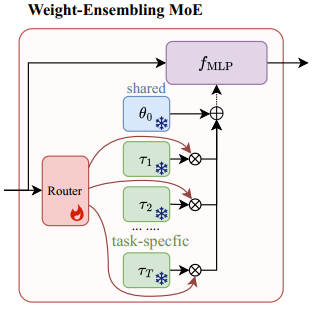
\includegraphics[height=3.7cm]{arch_wemoe_module}\\[-.5mm]
      {\tiny WEMoE module; here $T=5$\refm{2}}
    \end{column}
    \begin{column}{.62\linewidth}
      \[w^{\ell}(x)=\frac{1}{N}\sum_{j=1}^{N}r^{\ell}(h_j)\in\mathbb{R}^{5}\]
      \[W^{\ell}(x)=W_0^{\ell}+\sum_{e=1}^{5}w_e^{\ell}(x)\,\tau_e^{\ell}\]
      \[r^{\ell}(h)=\mathrm{fc}_2\big(\mathrm{ReLU}(\mathrm{fc}_1(h))\big)\]
    \end{column}
  \end{columns}
  \vfill
  \begin{itemize}\footnotesize
    \item One router per encoder layer; the mean runs over non-padding tokens; both MLP linear layers share $w^{\ell}$.
    \item No softmax: a weight can exceed 1 or be negative, so a router can amplify or subtract a task vector.
    \item The router's bias starts at $\lambda$, so the model starts close to Task Arithmetic.
  \end{itemize}
\end{frame}

\begin{frame}{Objective: few-shot fine-tuning (FSFT)}
  \textbf{Cross-entropy on a small labelled set, summed over the tasks:}
  \[
    \min_{\phi}\ \sum_{t=1}^{5}\ \frac{1}{|B_t|}\sum_{(x,y)\in B_t}-\log p_{\phi}(y\mid x,t),
    \qquad B_t\subset D_t^{(k)},\ \ |D_t^{(k)}|=k
  \]
  \begin{itemize}
    \item $\phi$: router parameters, \textbf{the only trainable weights} (7.1M).
    \item $D_t^{(k)}$: $k$ labelled examples of task $t$, which the experts have never seen.
    \item $p_{\phi}$: softmax over the logits of head $g_t$.
  \end{itemize}
  \vfill
  \centering
  \begin{tikzpicture}
    \node[frz,minimum width=2.9cm] (a) at (0,0) {$\tau_e$, $W_0$, non-MLP, heads\\ frozen};
    \node[trn,minimum width=2.4cm] (b) at (4,0) {Routers $\phi$\\ updated by gradient};
    \node[mix,minimum width=2.6cm] (c) at (8,0) {Best step\\ chosen on dev};
    \draw[flow] (a) -- (b);
    \draw[flow] (b) -- (c);
  \end{tikzpicture}
  \nextq{how does the whole pipeline run?}
\end{frame}
